\documentclass[11pt]{article}
\usepackage[margin=1in]{geometry}
\usepackage{amsmath,amssymb,bm}
\usepackage{physics}
\usepackage{graphicx}
\usepackage{hyperref}

\newcommand{\Jx}{J_x}
\newcommand{\Jy}{J_y}
\newcommand{\Jz}{J_z}
\newcommand{\Jp}{J_+}
\newcommand{\Jm}{J_-}
\newcommand{\dt}{\delta t}

\title{Open-system model for light-shift-driven multiparameter spin metrology}
\author{}
\date{}

\begin{document}
\maketitle

\section{Setup}

We consider a single spin $J$ (one atom of a product ensemble of $N_a$ atoms; for
$J=3$ this is the Cs $F=3$ hyperfine manifold) evolving under a closed-system Hamiltonian
that is the sum of a static field to be estimated, an rf control rotation with a
piecewise-constant random phase, and a nonlinear term generated by the tensor light shift
of an off-resonant, linearly polarized beam. With $\hbar = 1$ and time in units of
$1/\Omega$,
\begin{equation}
  H(t) \;=\; \underbrace{\bm{w}\cdot\bm{J}}_{\text{field to estimate}}
  \;+\; \underbrace{\Omega\big[\cos\phi(t)\,\Jx + \sin\phi(t)\,\Jy\big]}_{\text{rf control}}
  \;+\; \underbrace{\frac{\beta}{2J}\,\Jz^2}_{\text{tensor light shift}},
  \label{eq:H}
\end{equation}
where $\bm{w} = (w_x, w_y, w_z)$ is the three-component parameter vector and $\phi(t)$
is constant on blocks of \texttt{random\_phase\_steps} time steps and drawn uniformly on
$[0, 2\pi)$ for every realization. The code's parameter \texttt{beta} enters as
$\beta/2J$, as written.

\section{Light-induced decoherence}

The same beam that produces the $\Jz^2$ term scatters photons. In the far-detuned
limit (detuning large compared with the excited-state hyperfine splitting
$\Delta_{\mathrm{HF}}'$ but small compared with the fine-structure splitting) the
scattering amplitude acts on the electron spin alone. For linear polarization the
no-spin-flip (Rayleigh) part is a scalar and does not decohere the ground manifold. The
spin-flip (Raman) part, projected onto the $F$ manifold, is proportional to $J_\pm$ by
the Wigner--Eckart theorem. Neglecting Raman loss to the other hyperfine manifold and
any decoherence from a separate readout beam, the single decoherence channel is
therefore the pair of jump operators
\begin{equation}
  L_+ = \sqrt{\gamma}\,\Jp, \qquad L_- = \sqrt{\gamma}\,\Jm, \qquad J_\pm = \Jx \pm i\Jy .
  \label{eq:jumps}
\end{equation}

Both the tensor light shift and the scattering rate scale with intensity over detuning
squared, $\beta \propto I\,\Delta_{\mathrm{HF}}'/\Delta^2$ and
$\gamma_s \propto I\,\Gamma/\Delta^2$, so their ratio is a property of the atom and
the transition, not of the beam. We parametrize this by a fixed figure of merit
\begin{equation}
  \eta \equiv \frac{\beta}{\gamma}, \qquad \gamma = \frac{\beta}{\eta},
  \qquad \eta \sim c\,\frac{\Delta_{\mathrm{HF}}'}{\Gamma} = \mathcal{O}(10\text{--}100),
  \label{eq:eta}
\end{equation}
with $c$ an order-one Clebsch--Gordan factor obtainable from the ground-state
polarizability and optical-pumping formalism of Deutsch and Jessen
(Opt.\ Commun.\ \textbf{283}, 681 (2010)). Consequently the nonlinearity cannot be
increased without increasing the decoherence in proportion, and a sweep over $\beta$
is simultaneously a sweep over $\gamma$.

\section{Master equation (Schr\"odinger picture)}

The Lindblad master equation for the single-atom density matrix is
\begin{equation}
  \dv{\rho}{t} \;=\; -i\,[H(t), \rho]
  \;+\; \gamma\Big(\Jp \rho \Jm - \tfrac12\{\Jm\Jp, \rho\}\Big)
  \;+\; \gamma\Big(\Jm \rho \Jp - \tfrac12\{\Jp\Jm, \rho\}\Big).
  \label{eq:ME}
\end{equation}
Writing $J_\pm = \Jx \pm i\Jy$, the cross terms cancel and the dissipator collapses to
\begin{equation}
  \mathcal{D}[\rho] \;=\; 2\gamma \sum_{k=x,y}\Big(J_k \rho J_k - \tfrac12\{J_k^2, \rho\}\Big)
  \;=\; -\gamma\Big([\Jx,[\Jx,\rho]] + [\Jy,[\Jy,\rho]]\Big),
  \label{eq:D}
\end{equation}
a double-commutator (dephasing-type) channel along $x$ and $y$, each at rate $2\gamma$.
It commutes with rotations about $z$, conserves the trace, and is unital: the
maximally mixed state $\mathbb{1}/(2J+1)$ is its fixed point. Here
$\Jm\Jp + \Jp\Jm = 2(\Jx^2 + \Jy^2) = 2\big[J(J+1) - \Jz^2\big]$.

\section{Master equation (Heisenberg picture)}

Expectation values can equally be computed by propagating the observable with the
adjoint generator,
\begin{equation}
  \expval{O}(t) = \Tr\!\big[O\, e^{t\mathcal{L}}(\rho_0)\big]
                = \Tr\!\big[e^{t\mathcal{L}^\dagger}(O)\, \rho_0\big],
\end{equation}
with
\begin{align}
  \dv{O}{t} &= i\,[H(t), O]
  + \gamma\Big(\Jm O \Jp - \tfrac12\{\Jm\Jp, O\}\Big)
  + \gamma\Big(\Jp O \Jm - \tfrac12\{\Jp\Jm, O\}\Big) \notag \\
  &= i\,[H(t), O] - \gamma\Big([\Jx,[\Jx,O]] + [\Jy,[\Jy,O]]\Big).
  \label{eq:adjME}
\end{align}
The dissipator takes the same form in both pictures because the jump set
$\{\Jp, \Jm\}$ is closed under Hermitian conjugation. This is the form integrated in
the simulation: the observable $O = \Jy$ (or $\Jz$) is propagated and the signal is
$\Tr[O(t)\rho_0]$ with $\rho_0$ the initial spin coherent state.

\subsection*{Exact relaxation of the first moments}

Because $\mathcal{D}^\dagger$ maps the vector operator $\bm{J}$ onto itself,
\begin{equation}
  \mathcal{D}^\dagger[\Jx] = -\gamma\,\Jx, \qquad
  \mathcal{D}^\dagger[\Jy] = -\gamma\,\Jy, \qquad
  \mathcal{D}^\dagger[\Jz] = -2\gamma\,\Jz,
\end{equation}
so for any $J$ the Bloch vector obeys
\begin{align}
  \dv{t}\expval{\Jx} &= (\text{coherent}) - \gamma\expval{\Jx}, \\
  \dv{t}\expval{\Jy} &= (\text{coherent}) - \gamma\expval{\Jy}, \\
  \dv{t}\expval{\Jz} &= (\text{coherent}) - 2\gamma\expval{\Jz}.
\end{align}
The coherent part is not closed at first order because the $\Jz^2$ term couples
$\expval{\bm J}$ to second moments; it is handled numerically below. The parameter
$\gamma$ is therefore the transverse relaxation rate, and $2\gamma$ the longitudinal
one.

\section{Measurement model}

At each time step $n$ the recorded datum is
\begin{equation}
  M_n = \expval{O}_n + \xi_n, \qquad \xi_n \sim \mathcal{N}(0, \sigma^2), \qquad
  \sigma = \frac{1}{\sqrt{N_p}\, G\, N_a},
\end{equation}
i.e.\ the ensemble-averaged single-atom expectation value with Gaussian photon shot
noise from a separate readout beam of $N_p$ photons per step, Faraday gain $G$, and
$N_a$ atoms. Back-action of the readout beam is not included. The estimator is the
least-squares fit of $\bm w$ to $\{M_n\}$ using the same open-system forward model,
with $\gamma$ treated as known (it is fixed by the chosen $\beta$), and its
covariance is compared with the classical Cram\'er--Rao bound
$\mathrm{Cov}(\hat{\bm w}) \ge F^{-1}$,
\begin{equation}
  F_{ab} = \frac{1}{\sigma^2}\sum_n \pdv{\expval{O}_n}{w_a}\,\pdv{\expval{O}_n}{w_b}.
\end{equation}

\section{Numerical integration}

Time is discretized with step $\dt$. With $U_w = e^{-i\dt\,\bm w\cdot\bm J}$ and
$U_c[n] = e^{-i\dt\,H_c[n]}$ the control step for block $n$, define
$U_n = U_c[n]\,U_w$. The Hamiltonian and dissipative parts are split to first order,
\begin{align}
  \text{Schr\"odinger:}\qquad & \rho_{n+1} = e^{\dt\,\mathcal{D}}\big(U_n \rho_n U_n^\dagger\big), \\
  \text{Heisenberg:}\qquad & O_{n+1} = U_n^\dagger\, e^{\dt\,\mathcal{D}^\dagger}(O_n)\, U_n .
  \label{eq:trotter}
\end{align}
The map $A \equiv e^{\dt\,\mathcal{D}^\dagger}$ is built once per realization as a
$(2J+1)^2 \times (2J+1)^2$ matrix acting on the vectorized observable (the exact
solution of the dissipative part over one step), so no approximation beyond the
first-order splitting is made. That splitting is of the same order as the pre-existing
split between $U_w$ and $U_c$. Because $A$ is linear and independent of $\bm w$, the
Fr\'echet-derivative recursion for $\partial O_n/\partial w_a$, needed for the Fisher
matrix, is unchanged apart from passing $O_n$ and $\partial O_n/\partial w_a$ through
$A$ first. Setting $\gamma = 0$ (no \texttt{--eta}) recovers the closed-system code
exactly.

\paragraph{Expected consequence.} The signal derivatives $\partial\expval{O}_n/\partial w_a$
decay on the time scale $1/\gamma$, so the accumulated Fisher information saturates
near $T \sim 1/\gamma$ instead of growing polynomially. At a fixed total time $T$
the useful nonlinearity is bounded by $\beta \lesssim \eta/T$, and the question
becomes whether the nonlinearity improves multiparameter estimation enough to pay for
the decoherence it necessarily brings.

\section{Assumptions and how to relax them}

The model above rests on two simplifications, adopted deliberately for the first
study. Both can be removed within the same numerical scheme.

\subsection*{A1: the readout beam does not decohere the atoms}

\emph{Relaxed in Section~\ref{sec:onebeam} (script v6).}

The measurement model treats the $N_p$ readout photons per step as pure shot noise. A
readout beam scatters photons too, through the same Raman channel (\ref{eq:jumps}),
so it adds to $\gamma$ a rate $\gamma_r$ set by the readout intensity rather than by
$\beta$. Because Faraday signal and scattering both scale as $1/\Delta^2$, the ratio
of measurement signal-to-noise to scattering is independent of detuning and fixed by
the resonant optical depth $\mathrm{OD} = N_a\sigma_0/A$: up to order-one
polarization and branching factors, the number of photons scattered per atom over the
whole run is
\begin{equation}
  P_{\mathrm{sc}} \;\simeq\; \frac{\mathrm{SNR}^2_{\mathrm{tot}}}{N_a\,\mathrm{OD}},
  \qquad
  \mathrm{SNR}^2_{\mathrm{tot}} = G^2 N_a^2 N_p^{\mathrm{tot}} = \sum_n \sigma^{-2}
  \label{eq:Psc}
\end{equation}
per unit of $\expval{J}$. With the values used in the simulations
($G = 8.9\times10^{-7}$, $N_a = 2\times10^{5}$, $N_p^{\mathrm{tot}} = 9.6\times10^{8}$)
this gives $\mathrm{SNR}^2_{\mathrm{tot}} \approx 3\times10^{7}$ and hence
$P_{\mathrm{sc}} \sim 10^{2}/\mathrm{OD}$, i.e.\ $\gamma_r T \sim 10^{2}/\mathrm{OD}$.
For comparison the light-shift beam contributes $\gamma T = \beta T/\eta$, which for
$T = 14/\Omega$ and $\eta \sim 30$ is $\approx 0.5\,\beta$. So unless
$\mathrm{OD} \gtrsim 10^{3}$ (a cavity, or a very dense cloud), the readout beam
decoheres the atoms at least as strongly as the light-shift beam does for
$\beta \lesssim 1$, and assumption A1 is not self-consistent with the assumed
shot-noise level. Relaxing it costs one extra parameter, $\mathrm{OD}$, and one
change to the model: replace $\gamma \to \gamma + \gamma_r$ in (\ref{eq:jumps}) with
$\gamma_r = P_{\mathrm{sc}}/T$, independent of $\beta$. This also introduces the
usual continuous-measurement trade-off between $N_p$ and $\gamma_r$ that the present
model does not see. (In the single-beam scheme of Deutsch and Jessen the light-shift
and readout beams are the same beam, so $\beta$, $N_p$ and $\gamma$ are all tied to
one intensity.)

\subsection*{A2: no loss from the $F$ manifold}

\emph{Relaxed in Section~\ref{sec:loss} (script v7).}

The Raman process that gives (\ref{eq:jumps}) also transfers atoms to the other
ground hyperfine manifold ($F=4$ for Cs $F=3$) with a branching ratio of order one,
so loss occurs at a rate $\gamma_L \sim \gamma$. Within the $F$-manifold Hilbert
space this is a non-trace-preserving term
\begin{equation}
  \dv{\rho}{t} \supset -\tfrac12\{K_L, \rho\}, \qquad
  K_L = \sum_q L_q^{L\dagger} L_q^{L} = a + c\,\Jz^2 ,
\end{equation}
where $L_q^{L} \propto P_{F'} s_q P_F$ are the jump operators into $F'$ and the form
of $K_L$ follows from $z$-symmetry and the $m \to -m$ reflection symmetry of
$\pi$-polarized light. If the lost atoms are dark to the readout, the unnormalized
$\Tr[O\rho]$ is automatically the measured signal, and in the simplest uniform
approximation $K_L = \gamma_L\mathbb{1}$ this is just a known factor
$e^{-\gamma_L t}$ multiplying the signal and its derivatives. In the code this is one
additional $w$-independent factor per step, so the fit and Fisher recursion are again
unchanged. The complication that this approximation hides is that atoms in $F'$ are
not dark: they Faraday-rotate the readout with a different (roughly opposite) sign and
evolve under a different light shift. Treating that properly requires enlarging the
state space to $F \oplus F'$ (dimension $16$ for Cs), which the superoperator scheme
of Section 6 supports at the cost of a $256\times256$ dissipative map.


\section{One beam: light shift, decoherence and readout from the same probe}
\label{sec:onebeam}

In the actual scheme there is a single off-resonant, linearly polarized probe. It produces
the tensor shift, it scatters photons, and its Faraday rotation is the readout. With photon
flux $\Phi$ and detuning $\Delta$, in the far-detuned limit,
\begin{equation}
  \beta \propto \frac{\Phi\,\Delta_{\mathrm{HF}}'}{\Delta^{2}}, \qquad
  \gamma \propto \frac{\Phi\,\Gamma}{\Delta^{2}}, \qquad
  G \propto \frac{1}{\Delta}, \qquad
  \sigma^{2} = \frac{1}{N_p G^{2} N_a^{2}} \propto \frac{\Delta^{2}}{\Phi},
\end{equation}
where $G$ is the rotation per atom per unit spin and $N_p \propto \Phi$ the photons per
measurement interval $\dt$. All four depend on $\Phi$ and $\Delta$ only through
$\Phi/\Delta^{2}$, so the probe strength is a single knob and two ratios are fixed by the
physics:
\begin{equation}
  \frac{\beta}{\gamma} = \eta, \qquad
  \gamma\,\sigma^{2}\,\dt = \frac{1}{\mathrm{OD}_{\mathrm{eff}}\,N_a},
  \qquad \mathrm{OD}_{\mathrm{eff}} = c\,\frac{N_a\sigma_0}{A},
  \label{eq:onebeam}
\end{equation}
with $c$ an order-one factor from the vector polarizability and the spin-flip branching
ratio. The second relation is the readout back-action of Section~7 made exact: the
photons that carry the Faraday signal are the photons that scatter. Taking $\beta$ as the
sweep variable, the script \texttt{v6} derives per $\beta$
\begin{equation}
  \gamma = \frac{\beta}{\eta}, \qquad
  \sigma(\beta) = \sqrt{\frac{\eta}{\mathrm{OD}_{\mathrm{eff}}\,N_a\,\dt\,\beta}} .
  \label{eq:onebeam-derived}
\end{equation}
A stronger probe brings more nonlinearity, more decoherence and \emph{less} shot noise;
$\beta \to 0$ is no light at all, with no decoherence but no measurement either, so
$\beta = 0$ is excluded from the sweep and there is no decoherence-free reference. The
former constants $G$ and $N_p$ are absorbed into $\mathrm{OD}_{\mathrm{eff}}$; with the
values used in v4/v5 and $\eta = 30$, $\mathrm{OD}_{\mathrm{eff}} = 10$, the old noise level
$\sigma = 0.021$ corresponds to $\beta \approx 33$, a far stronger probe than any $\beta$
in the v5 sweep. The two physics inputs are now $\eta$ (atom) and $\mathrm{OD}_{\mathrm{eff}}$
(sample); both are placeholders in the launcher until derived and measured.

\paragraph{Expected shape of the optimum.} The Fisher information per step is
$(\partial\expval{O}/\partial w)^2/\sigma^2 \propto \beta\,(\partial\expval{O}/\partial w)^2$,
and the derivative decays on the scale $\eta/\beta$. For $T \ll \eta/\beta$ the information
grows like $\beta\,T^{3}$ (more probe is better), for $T \gg \eta/\beta$ it saturates like
$\eta^{3}/\beta^{2}$ (less probe is better), so the optimum sits at a finite
$\beta_{\rm opt} \sim \eta/T$ for every $T$. Unlike v5, where $\beta = 0$ eventually won
because it was decoherence-free, the one-beam model always has a nonzero optimal probe
strength.

\paragraph{Control experiment.} Because the nonlinearity cannot be switched off physically
without switching off the probe, \texttt{v6} has a flag \texttt{--tensor-scale} that
multiplies the $J_z^2$ term in the Hamiltonian only, keeping the beam-derived $\gamma$ and
$\sigma$. Running the same sweep with \texttt{--tensor-scale 0} isolates what the nonlinear
dynamics contributes to the estimation at fixed decoherence and fixed shot noise.


\section{Loss, and the light-induced coefficients from atomic structure}
\label{sec:loss}

The coefficients that Sections~2 and~\ref{sec:onebeam} left as placeholders ($\eta$, the
order-one factors in $\mathrm{OD}_{\mathrm{eff}}$) follow from the atomic structure. The
script \texttt{cs\_light\_shift\_scattering\_ratios.py} builds, for Cs ($I = 7/2$) on the
D1 or D2 line and a $\pi$-polarized far-detuned probe, the ground-state light-shift
operator and the optical-pumping jump operators by adiabatic elimination of the excited
manifold (Steck matrix elements, closure and normalization checked, vector-to-scalar
polarizability ratio converging to $\pm 1/4$ on D1 and $\pm 1/8$ on D2). Writing
$\gamma_s$ for the total photon scattering rate of the spin coherent state, the far-detuned
values are
\begin{center}
\begin{tabular}{lccccc}
\hline
line, $F$ & $\eta_s = \beta/\gamma_s$ & $r_{\rm within}$ & $K_L/\gamma_s = a_L + c_L m^2$ & $b/a$ & $\eta_{\rm tot} = \beta/R_{\rm tot}$ \\
\hline
D2, $F=3$ & $7.4$   & $0.0055$ & $0.204 + 0.0107\,m^2$ & $0.127$  & $33$   \\
D2, $F=4$ & $-9.5$  & $0.0052$ & $0.130 + 0.0104\,m^2$ & $-0.123$ & $-61$  \\
D1, $F=3$ & $-100$  & $0.0110$ & $0.412 + 0.0264\,m^2$ & $-0.243$ & $-217$ \\
D1, $F=4$ & $122$   & $0.0115$ & $0.254 + 0.0170\,m^2$ & $0.257$  & $408$  \\
\hline
\end{tabular}
\end{center}
Here $r_{\rm within}\gamma_s$ is the rate of the within-manifold spin-flip channel
(\ref{eq:jumps}), $K_L$ the rate operator of Raman transfer out of the manifold, $b/a$ the
vector-to-scalar polarizability ratio per unit $m$ that sets the Faraday signal, and
$R_{\rm tot} = r_{\rm within}\gamma_s + \expval{K_L}$ the initial relaxation rate of
$\expval{F_x}$. A negative $\eta_s$ is a tensor shift of the opposite sign. Two things stand
out: the relaxation is 96--98\,\% loss and only a few per cent spin flips, so the channel of
Sections~2--5 is the minor one; and $\eta_{\rm tot} = 33$ for D2, $F=3$ is essentially the
placeholder $\eta = 30$ used so far, while D1, $F=4$ offers twelve times more nonlinearity
per unit of relaxation.

\paragraph{Master equation with loss.} The loss adds a trace-decreasing term with no jump
operator, since the atom leaves the manifold:
\begin{equation}
  \dv{\rho}{t} = -i[H,\rho] + \mathcal{D}_{\rm sf}[\rho] - \tfrac12\{K_L,\rho\},
  \qquad
  \dv{O}{t} = i[H,O] + \mathcal{D}^\dagger_{\rm sf}[O] - \tfrac12\{K_L,O\},
  \qquad K_L = \gamma_s\big(a_L + c_L \Jz^2\big),
\end{equation}
with $\mathcal{D}_{\rm sf}$ the channel (\ref{eq:D}) at rate $r_{\rm within}\gamma_s$. The
step map $A = e^{\dt\,\mathcal{D}^\dagger}$ of Section~6 absorbs both terms and stays
$\bm w$-independent; on the identity it acts as $e^{-\dt K_L}$, so $\Tr[O(t)\rho_0]$ is the
survival probability times the conditional expectation, which is the collective Faraday
signal if lost atoms are dark. Survivors evolve coherently: loss only scales the signal,
unlike the spin-flip channel that scrambles it. The remaining approximation of the light
model is that atoms transferred to $F'$ are not in fact dark; they carry a vector response
of opposite sign and a different light shift.

\paragraph{Parametrization (script v7).} With the probe strength swept as $\beta$,
\begin{equation}
  \gamma_s = \frac{\beta}{|\eta_s|}, \qquad
  \gamma_{\rm sf} = r_{\rm within}\gamma_s, \qquad
  K_L = \gamma_s(a_L + c_L\Jz^2), \qquad
  \sigma^2 = \frac{1}{(b/a)^2\,\mathrm{OD}_{\rm res}\,N_a\,\dt\,\gamma_s},
\end{equation}
where $\mathrm{OD}_{\rm res} = N_a\sigma_{\rm res}/A$ is the resonant optical depth of the
probe transition, the only sample input besides $N_a$. In terms of Section~\ref{sec:onebeam},
$\mathrm{OD}_{\rm eff} = (b/a)^2\,\mathrm{OD}_{\rm res}/(R_{\rm tot}/\gamma_s)$, which is
$0.07$ (D2, $F=3$) to $0.22$ (D1, $F=4$) of $\mathrm{OD}_{\rm res}$. The
$\mathrm{OD}_{\rm eff} = 10$ of the first one-beam run therefore corresponds to
$\mathrm{OD}_{\rm res} \approx 140$; a free-space cloud of $2\times10^5$ atoms in a 50\,$\mu$m
beam has $\mathrm{OD}_{\rm res}$ of order 6--9; both were run (Section~\ref{sec:results}).

\paragraph{Cram\'er--Rao bookkeeping.} The simulation fits every realization on its own
control sequence. The bound that such an estimator can reach, averaged over realizations,
is $\mathbb{E}[F_i^{-1}]$, not $[\mathbb{E}F_i]^{-1}$ (Jensen); with strong decoherence
the information comes from a short window in which the particular control phases matter,
and the two differ by an order of magnitude (a factor 17 at $\beta = 20$, $\eta = 30$).
Scripts v6 and v7 save both; the v7 runs confirm that the estimator reaches
$\mathbb{E}[F_i^{-1}]$ to within a few per cent once its fits have converged (Section~\ref{sec:results}).


\section{Results of the simulations}
\label{sec:results}

All runs use $J = 3$, observable $\Jy$, $T = 14/\Omega$, 300 fits per ($\beta$, cutoff) with 40
cutoffs, and 20 independent draws of $\bm w_{\rm true}$ (one per cluster array task); statistics
are averaged over the 20 draws. Fits whose least-squares cost lies above the $5\sigma$ chi-square
band (a few per cent, converged to a local minimum) are dropped before variances are formed.
``Variance'' below is the total filtered Monte Carlo variance $\mathrm{tr}\,\mathrm{Cov}(\hat{\bm w})$.

\begin{center}
\small
\begin{tabular}{llllll}
\hline
run & script & light model & atom / $\eta$ & OD & $\beta$ \\
\hline
\texttt{decoherence\_1} & v5 & spin flips, separate readout & $\eta = 30$ & -- ($\sigma = 0.021$) & $0$--$5$ \\
\texttt{onebeam\_1} & v6 & spin flips, one beam & $\eta = 30$ & $\mathrm{OD}_{\rm eff} = 10$ & $0.5$--$20$ \\
\texttt{loss\_1} & v7 & loss + spin flips, one beam & Cs D2 $F=3$ & $\mathrm{OD}_{\rm res} = 140$ & $0.5$--$20$ \\
\texttt{loss\_1\_od10} & v7 & same & same & $\mathrm{OD}_{\rm res} = 10$ & $0.5$--$20$ \\
\texttt{*\_notensor} & v7 & same beam, $\Jz^2$ off & same & 140 and 10 & $0.5$--$20$ \\
\hline
\end{tabular}
\end{center}

\paragraph{v5, separate readout.} With $\beta = 0$ a decoherence-free closed system, strong
nonlinearity wins only at short times: $\beta = 5$ reaches a variance of $10^{-2}$ at
$\Omega t = 1.15$ against $1.52$ for $\beta = 0$, and $10^{-3}$ at $1.86$ against $2.23$, but
its bound saturates at $\sim 10^{-5}$ while the closed system keeps improving, so for
$T \gtrsim 4/\Omega$ the best $\beta$ is $0$. This is the $\beta_{\rm opt} \sim \eta/T$ picture,
and it is the most pessimistic case for the nonlinear protocol because the reference carries no
decoherence at all.

\paragraph{v6, one beam.} With $\beta = 0$ excluded the optimum is finite at every $T$: by the
bound the best $\beta$ steps $20 \to 10 \to 5 \to 2 \to 1 \to 0.5$ at
$\Omega t = 0.5, 0.9, 1.3, 2.7, 6.7$. This run also exposed the Cram\'er--Rao bookkeeping issue of
Section~\ref{sec:loss}: at $\beta \ge 5$ the Monte Carlo variance sat 20--50 times above
$[\mathbb{E}F]^{-1}$ with no rejected fits and zero excess cost, which is not optimizer failure
but the Jensen gap, $\mathbb{E}[F_i^{-1}]/\mathrm{tr}[\mathbb{E}F]^{-1} = 2.4, 3.5, 17$ at
$\beta = 2, 5, 20$.

\paragraph{v7, loss: the estimator reaches its bound.} In \texttt{loss\_1} the ratio of the
Monte Carlo variance to $\mathrm{tr}\,\mathbb{E}[F_i^{-1}]$ at $T$ is $0.99$--$1.03$ for every
$\beta$; the least-squares estimator with random control is efficient once its fits have converged
(Fig.~\ref{fig:overview}). The tensor-off references are efficient at weak probe but sit above
their own reachable bound at strong probe ($17\times$ at $\beta = 20$ for $\mathrm{OD}_{\rm res} =
140$; $5$--$90\times$ for $\beta \ge 5$ at $\mathrm{OD}_{\rm res} = 10$), an identifiability
problem of the purely linear dynamics that only makes the reference worse where the nonlinear
run is already far ahead.

\begin{figure}[htbp]
\centering
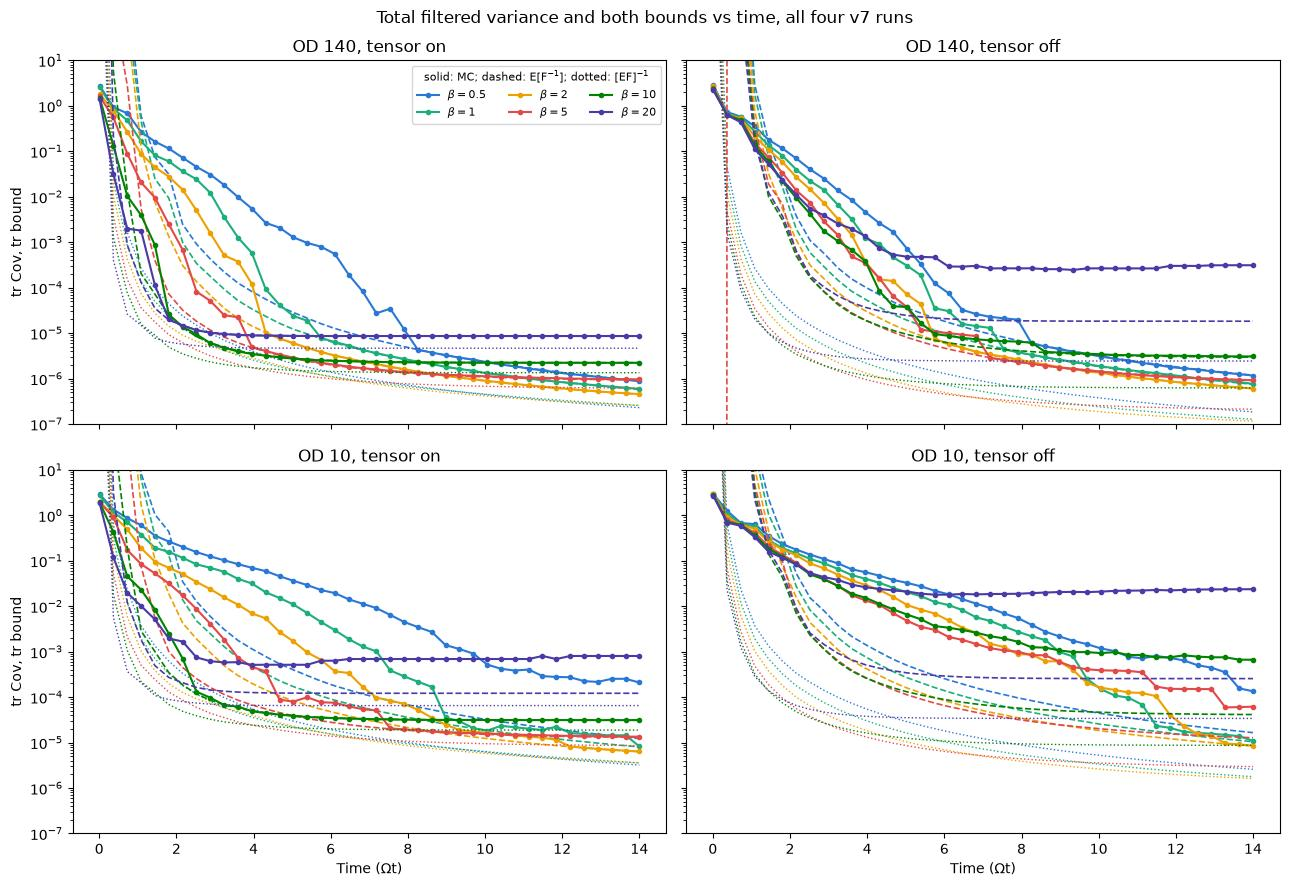
\includegraphics[width=\textwidth]{figures/v7_overview.pdf}
\caption{Total filtered Monte Carlo variance (solid), reachable bound $\mathrm{tr}\,\mathbb{E}[F_i^{-1}]$
(dashed) and naive bound $\mathrm{tr}\,[\mathbb{E}F]^{-1}$ (dotted) versus time for the four v7 runs.
Left: with the $\Jz^2$ term; right: identical beam without it. Top: $\mathrm{OD}_{\rm res} = 140$;
bottom: $10$.}
\label{fig:overview}
\end{figure}

\paragraph{v7: the nonlinearity helps, and by a lot.} The tensor-off runs share seeds, decoherence
and shot noise with the tensor-on runs, so the comparison is paired. Table~\ref{tab:ttt} gives, per
run and target variance, the earliest time after which the variance stays below the target
(minimized over $\beta$) and the $\beta$ that achieves it. Every target is reached three to four
times sooner with the nonlinearity, at both optical depths.

\begin{table}[htbp]
\centering
\begin{tabular}{lccccc}
\hline
target $\mathrm{tr}\,\mathrm{Cov}$ & $10^{-2}$ & $10^{-3}$ & $10^{-4}$ & $10^{-5}$ & $10^{-6}$ \\
\hline
$\mathrm{OD}_{\rm res}=140$, $\Jz^2$ on  & $0.52$ ($\beta{=}20$) & $1.16$ ($20$) & $1.47$ ($20$) & $2.46$ ($10$) & $9.55$ ($2$) \\
$\mathrm{OD}_{\rm res}=140$, $\Jz^2$ off & $2.13$ ($10$) & $3.28$ ($10$) & $4.27$ ($10$) & $5.69$ ($2$) & $11.21$ ($2$) \\
$\mathrm{OD}_{\rm res}=10$, $\Jz^2$ on   & $1.09$ ($20$) & $2.06$ ($10$) & $2.85$ ($10$) & $11.99$ ($2$) & -- \\
$\mathrm{OD}_{\rm res}=10$, $\Jz^2$ off  & $4.37$ ($5$) & $7.77$ ($2$) & $10.67$ ($1$) & $13.24$ ($2$) & -- \\
\hline
\end{tabular}
\caption{Time ($\Omega t$) after which the total filtered variance stays below the target, best over
$\beta$ (the optimal $\beta$ in parentheses); -- = not reached within $T = 14/\Omega$.}
\label{tab:ttt}
\end{table}

At equal $\beta$ the ratio of variances with and without the $\Jz^2$ term (Fig.~\ref{fig:onoff})
is $0.05$, $0.0015$ and $0.0013$ at $\Omega t = 2$ for $\beta = 5, 10, 20$
($\mathrm{OD}_{\rm res} = 140$), still $0.35$ and $0.03$ at $\Omega t = 8$ for $\beta = 10, 20$,
and $0.03$ at $T$ for $\beta = 20$; for $\beta \le 2$ it is $0.3$--$0.8$ throughout. The ratio of
the reachable bounds tells the same story ($0.02$--$0.06$ at $\Omega t = 2$ for $\beta \ge 5$,
$0.5$--$0.8$ at $T$) and is independent of $\mathrm{OD}$, since $\sigma^2$ is a common factor. The
naive bound $[\mathbb{E}F]^{-1}$ says the opposite, a ratio of $1.2$--$2.9$ at $T$: the nonlinear
dynamics make the information depend more strongly on the particular random control, which
enlarges the Jensen gap and which a fixed-control bound cannot see. The mechanism is the one
anticipated in Section~\ref{sec:onebeam}: the nonlinearity converts the probe into information
faster, so a target precision is reached before the loss has eaten the signal. The best $\beta$
by Monte Carlo falls with the time budget, $20$ up to $\Omega t \approx 2$, $10$ to $\approx 5$,
$5$ to $\approx 9$, then $2$, in agreement with $\beta_{\rm opt} \sim \eta_{\rm tot}/T$ up to a
prefactor.

\begin{figure}[htbp]
\centering
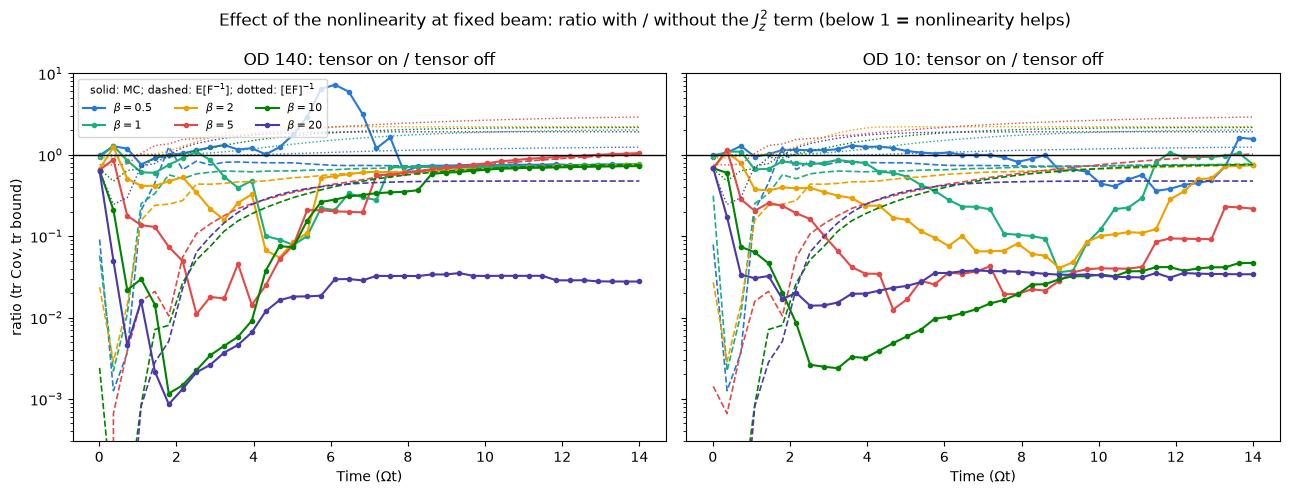
\includegraphics[width=\textwidth]{figures/v7_tensor_on_off.pdf}
\caption{Effect of the nonlinearity at fixed beam: ratio of the run with the $\Jz^2$ term to the run
without it, versus time and per $\beta$. Solid: Monte Carlo variance; dashed: reachable bound;
dotted: naive bound. Below 1 the nonlinearity helps.}
\label{fig:onoff}
\end{figure}

\paragraph{v7: loss is the gentler decoherence.} \texttt{loss\_1} and \texttt{onebeam\_1} have the
same $\beta$ list, the same nonlinearity per unit of initial signal relaxation
($\eta_{\rm tot} \approx 30$) and shot noise equal to within 5\,\%. They differ only in what the
scattering does to the atoms. With loss-dominated relaxation the variance at $T$ is lower by a
factor $0.84$, $0.44$, $0.075$ at $\beta = 0.5, 1, 2$ and by three orders of magnitude at
$\beta \ge 5$ (Fig.~\ref{fig:lossvssf}). Survivors keep evolving coherently and only the signal
amplitude decays, so the strong-probe regime that looked hopeless under the spin-flip model is
usable. Since loss is 97\,\% of the real relaxation for Cs, the v5/v6 picture overstated the cost
of the probe by a large factor.

\begin{figure}[htbp]
\centering
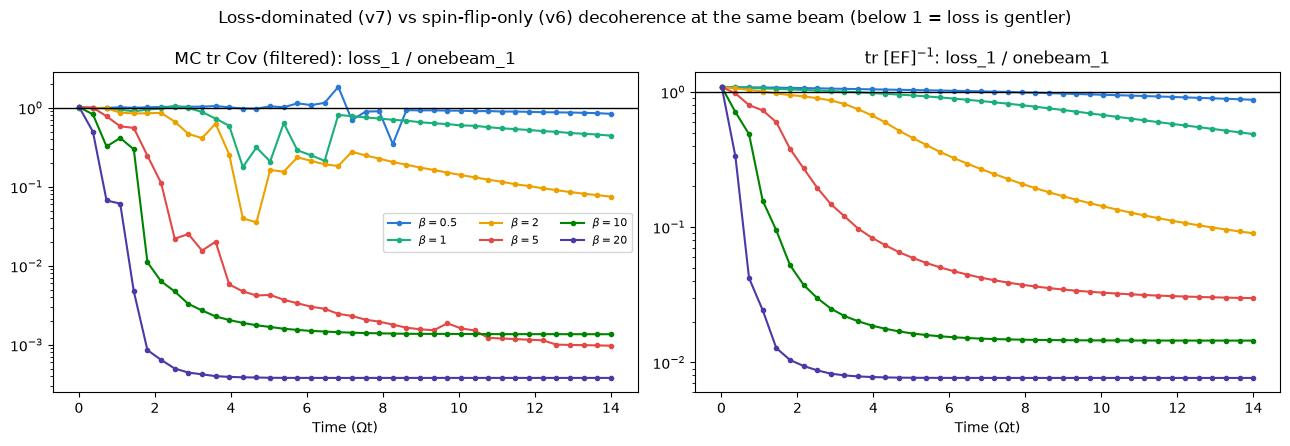
\includegraphics[width=\textwidth]{figures/v7_loss_vs_spinflip.pdf}
\caption{Loss-dominated (v7, \texttt{loss\_1}) versus spin-flip-only (v6, \texttt{onebeam\_1})
decoherence at the same beam: ratio of Monte Carlo variances (left) and of naive bounds (right).}
\label{fig:lossvssf}
\end{figure}

\paragraph{v7: free-space optical depth.} At $\mathrm{OD}_{\rm res} = 10$ the shot noise is
$3.7$ times larger and the variances at $T$ about ten times larger ($8\times10^{-6}$ against
$6\times10^{-7}$ at $\beta = 1$); the tightest target is out of reach within the run, but the
ordering of $\beta$ and the gain from the nonlinearity are unchanged (Table~\ref{tab:ttt}).

\paragraph{What remains.} (i) Atoms transferred to $F'$ are treated as dark; they carry a vector
response of opposite sign and a different light shift, and a faithful treatment needs the
$F \oplus F'$ space. (ii) The tensor-off reference at strong probe does not reach its own bound;
whether that is an optimizer or an identifiability limit of the linear dynamics is untested and
does not affect the conclusions. (iii) Cs D1, $F = 4$ offers $\eta_{\rm tot} = 408$, twelve times
more nonlinearity per unit of relaxation than the D2, $F = 3$ case run here, at the cost of
$J = 4$. (iv) The runs fix $T$ and sweep $\beta$; the experimental question is the converse, the
shortest $T$ for a required precision, which Table~\ref{tab:ttt} answers only on the $\beta$ grid.

\end{document}
